\section[MODELO DE ARQUITETURA]{MODELO DE ARQUITETURA}

O modelo de arquitetura no seu nível mais elevado, pode ser visto como um modelo de três camadas, conforme a Figura \ref{camadas_arquitetura}.
\begin{figure}[ht]
	\centering
	\includegraphics[width=7cm]{figuras/camadas.eps}
	\caption{Camadas arquiteturais.}
	\label{camadas_arquitetura}
\end{figure}

A camada \emph{web} é responsável pela interação com o usuário. 
A camada \emph{Web API} é responsável pela lógica de negócio. 
A camada de base de documentos é responsável pela persistência dos dados da aplicação.


\subsection[CAMADA DE APLICAÇÃO WEB] {CAMADA DE APLICAÇÃO WEB}
Esta camada foi projetada para rodar em \emph{browsers} que suportam \emph{HTML} 5. 
Ela é desenvolvida usando-se \emph{Javascript}, \emph{CSS} e \emph{HTML}. 
Além disso, adotou-se o \emph{framework} de desenvolvimento \emph{web} \emph{AngularJS}, ver \ref{angularjs}. 

Como o projeto não possuía recursos adequados a criação de uma equipe de desenvolvimento \emph{web} completa, afim de se minimizar os problemas com \emph{design web}, optou-se por usar a biblioteca \emph{angular-material}, ver \ref{angular_material}. 

A Figura \ref{material_amostra}, mostra um exemplo de uma tela criada com as diretivas do angular-material. Note que todo o \emph{look and feel} da tela é determinado pelo comportamento padrão da biblioteca.

\begin{figure}[H]
	\centering
	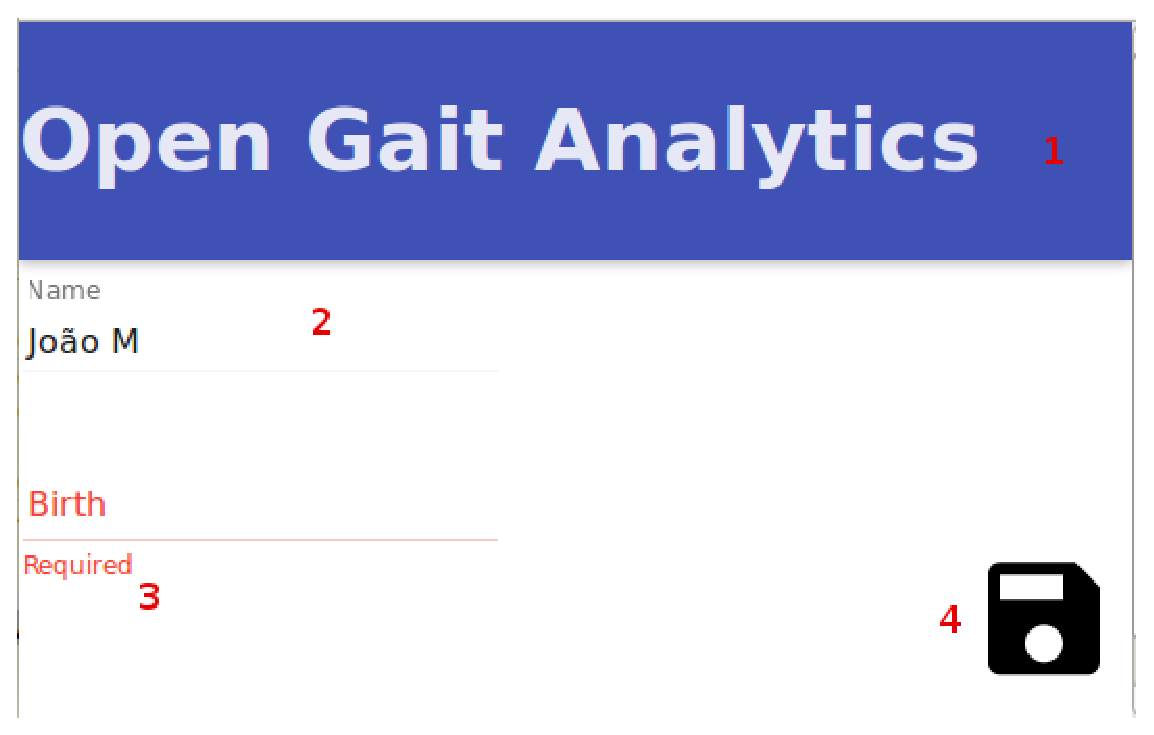
\includegraphics[width=9cm]{figuras/material_amostra.eps}
	\caption[Exemplo de uma tela criada com \emph{angular-material}.]{Exemplo de uma tela criada com \emph{angular-material}. 1) Diretiva \emph{md-toolbar}; 2) Diretiva \emph{md-input-container}; 3) Diretiva \emph{ng-messages} em conjunto com a \emph{md-input-container}; 4) Diretiva \emph{md-button}.}
	\label{material_amostra}
\end{figure}

\textbf{ORGANIZAÇÃO DO CÓDIGO FONTE}

\noindent
A criação de um ambiente de desenvolvimento \emph{web}, para um software de média para grande complexidade, não é uma tarefa trivial de ser resolvida.
É necessário criar padrões de organização de arquivos, configurar e instalar pacotes de software para desenvolvimento, testes, implantação, construção de \emph{builds}, entre outros.
Para facilitar esta tarefa, optou-se em utilizar o projeto \emph{angular-seed}, ver \ref{angular_seed}.
A ideia deste projeto é servir de esqueleto de projetos \emph{web} que utilizam o \emph{framework} \emph{AngularJS}.
Para usar este projeto, basta cloná-lo diretamente do seu repositório \emph{git} no \emph{site} github.com, conforme o comando abaixo.
\lstset{language=bash}
\begin{lstlisting}[frame=single]
git clone https://github.com/angular/angular-seed.git
\end{lstlisting}

\textbf{VISÃO ARQUITETURAL DA CAMADA \emph{WEB}}


\noindent
A Figura \ref{camda_web} mostra o funcionamento e os padrões mínimos a serem seguidos para implementação da camada \emph{web}.

\begin{figure}[H]
	\centering
	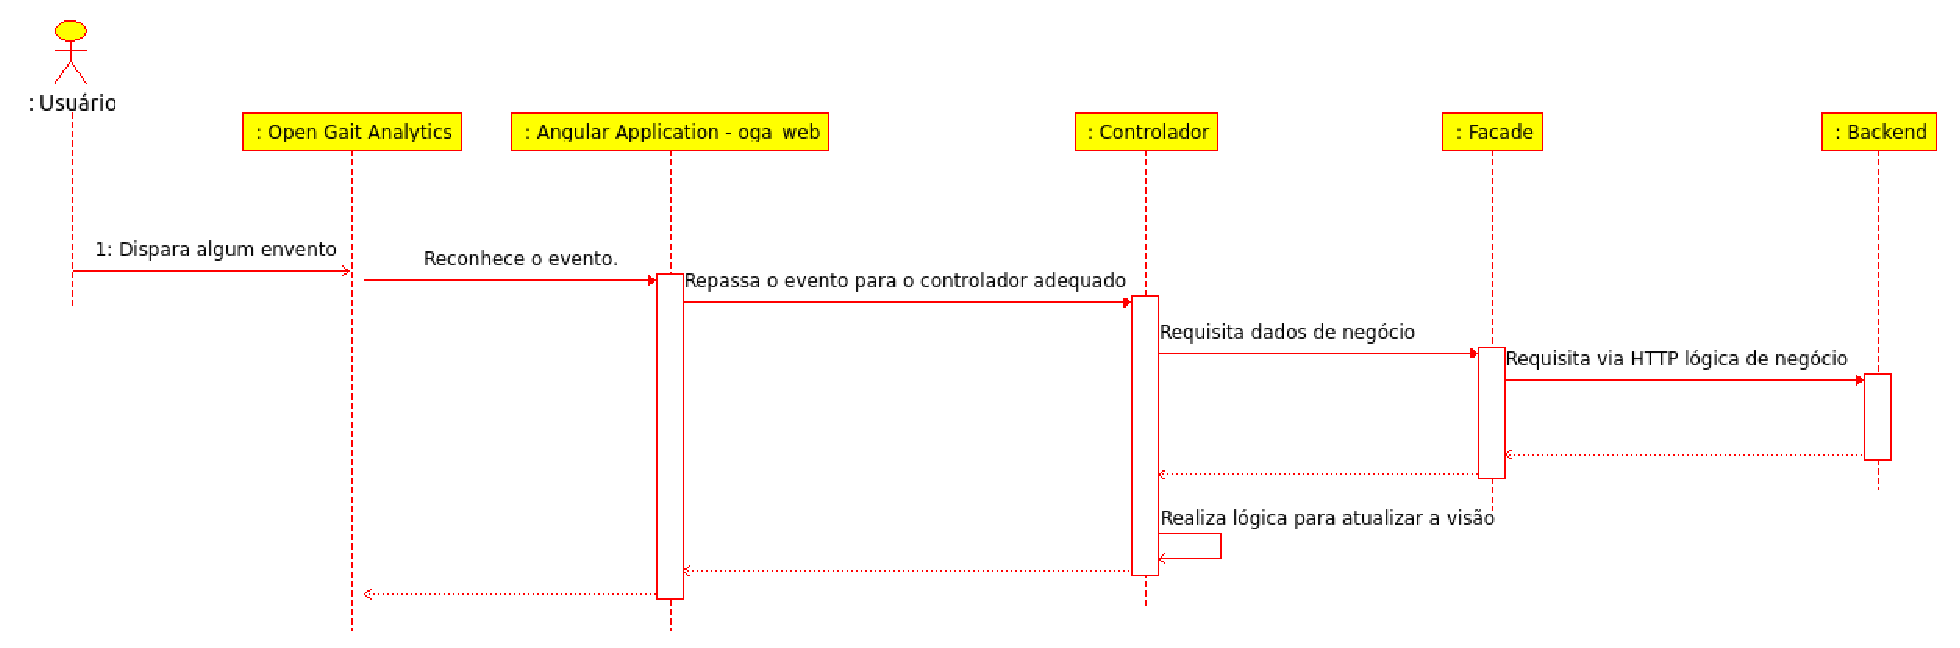
\includegraphics[width=17cm]{figuras/camada_web.eps}
	\caption{Camada \emph{web}.}
	\label{camda_web}
\end{figure}

Este esquema funciona da seguinte forma: O usuário usando seu \emph{browser}, acessa o \emph{site} do software. 
Ao realizar qualquer evento na aplicação, por exemplo, clicar num botão, ou selecionar um item em uma lista de seleção, a aplicação \emph{angularjs} detecta o evento e seleciona um componente de software chamado controlador. 
Existem vários destes controladores no sistema, cada evento do usuário é redirecionado para um que seja adequado.
No controlador é onde grande parte da programação acontece. 
Ele é associado a um \emph{template HTML}. 
Este template funciona como componente de apresentação para o usuário, e é o que o controlador manipula para mostrar informações ao usuário.
Quando o controlador precisa executar lógica de negócio, ou requisitar dados persistidos, ele deve chamar um componente do tipo \emph{Facade}. 
A aplicação \emph{web} roda no \emph{browser} do usuário e não persiste dados nem executa lógica de negócio. 
Este é um estilo arquitetural escolhido para o projeto.
A \emph{Facade} é um \emph{proxy} que se comunica com um \emph{backend} via HTTP no estilo \emph{REST} de comunicação via \emph{web}.

A Figura \ref{web_components}, mostra um exemplo de componentes escritos em \emph{JavaScript} respondendo a um evento disparado pelo usuário. 
Este evento poderia ser oriundo de um clique num botão ou na chamada de uma \emph{URL} específica. 
Depois de reconhecido o evento, no caso um pedido para ver a lista de pacientes, o componente \emph{PatientesCtrl} e o \emph{template patients.html} são carregado pelo \emph{framework AngularJS}. 
Neste momento o \emph{framework} acessa o componente \emph{PatientsFacade} através do seu método \emph{getPatients}. 
Este método invoca o método \emph{get} do componente \emph{\$HTTP} que faz parte do \emph{framework}.
Uma requisição é feita para o \emph{backend}, que retorna os dados no formato \emph{JSON}.
Finalmente, o \emph{framework} detecta a resposta e atualiza a tela para o usuário.

\begin{figure}[H]
	\centering
	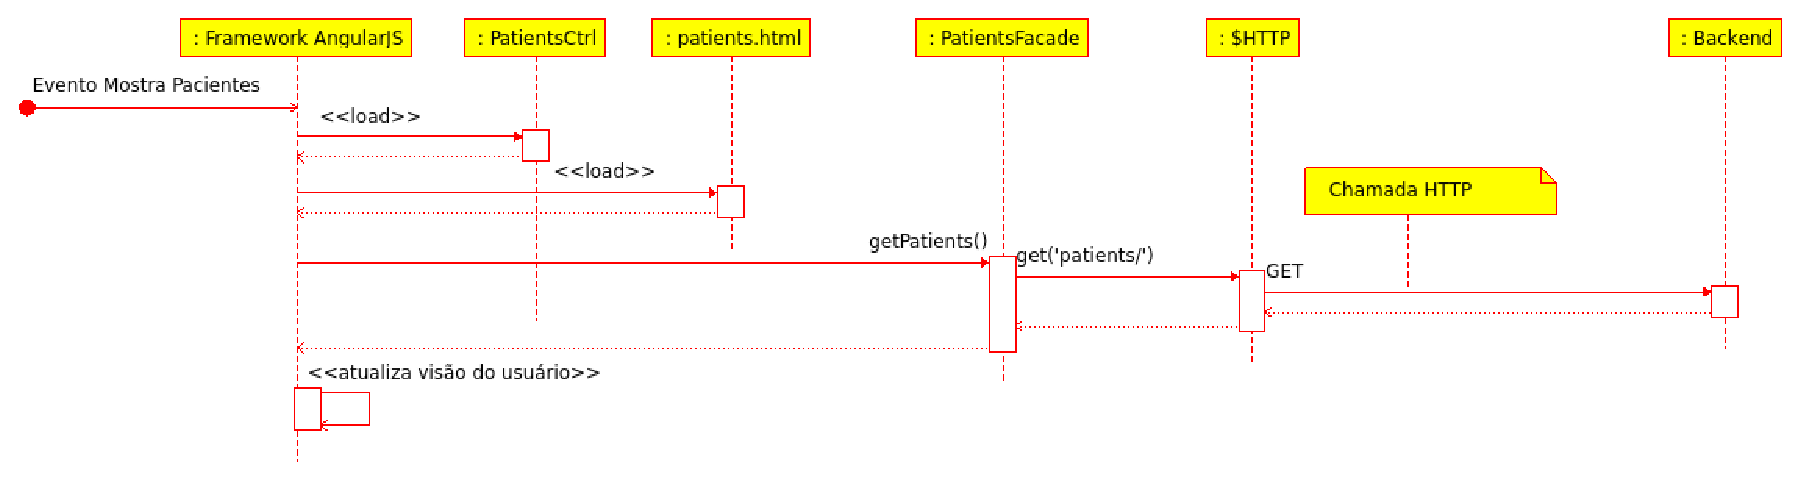
\includegraphics[width=17cm]{figuras/web_componentes.eps}
	\caption{Exemplo de componentes da camada \emph{web} funcionando juntos.}
	\label{web_components}
\end{figure}


\subsection{CAMADA \emph{REST WEB API}}

Esta é a camada responsável por expor toda a lógica de negócio e acesso a dados persistidos. Escolheu-se que esta camada fornece suas funções via \emph{web API} no estilo REST.
Uma das vantagens desta escolha é o alto desacoplamento, entre camada \emph{web} e lógica de negócio. 
Além disso, pode-se integrar mais facilmente a aplicação com outras, já que a lógica de negócio é toda exposta como \emph{API web}. 
Veja a seção \ref{servicos_rest} para um melhor entendimento deste estilo \emph{REST}.

\textbf{ORGANIZAÇÃO DO CÓDIGO FONTE}

\noindent
A Figura \ref{dir_api} mostra a configuração básica dos arquivos e diretórios da aplicação.

\begin{figure}[ht]
	\centering
	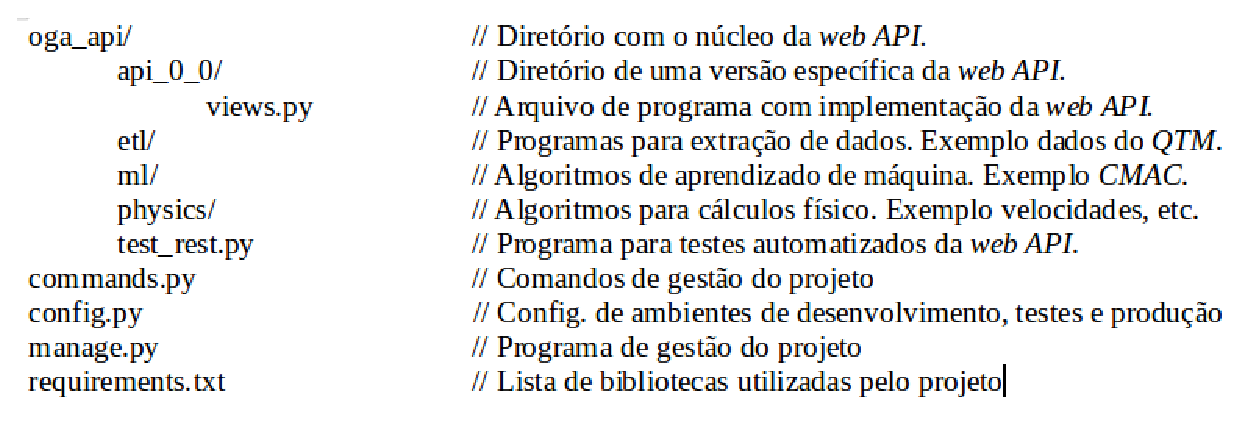
\includegraphics[width=15cm]{figuras/dir_api.eps}
	\caption{Organização do arquivos e diretórios da camada \emph{web API}.}
	\label{dir_api}
\end{figure}

A linguagem de programação \emph{Python} foi escolhida para implementar esta camada. Vários foram os motivos: a biblioteca \emph{Flask} para implementar a \emph{web API}, a biblioteca \emph{NumPy}, que é excelente para cálculos, comparável ao Matlab, a biblioteca \emph{Matplotlib} para criação de gráficos científicos, a baixa curva de aprendizado da linguagem, sua fama com desenvolvedores ao redor do mundo.

Para diminuir os problemas de ambientes, oriundos de um projeto complexo como este, optou-se por utilizar o programa \emph{virtualenv}. Este programa cria um ambiente \emph{python} virtual, baseado num arquivo de configuração. Isso faz com que todos os desenvolvedores envolvidos no projeto, possuam ambientes muito semelhantes.
Ao se clonar o projeto basta entrar no diretório da API e digitar o comando:
\lstset{language=bash}
\begin{lstlisting}[frame=single]
virtualenv env
\end{lstlisting}

Este comando irá criar uma diretório chamado \emph{env}. Para poder ativar o ambiente virtual é necessário o comado no unix:
\lstset{language=bash}
\begin{lstlisting}[frame=single]
. env/bin/activate
\end{lstlisting}

As bibliotecas necessárias a execução da aplicação estão listadas no arquivo \emph{requirements.txt}. Para instalá-las no novo ambiente virtual é necessário o comando:
\lstset{language=bash}
\begin{lstlisting}[frame=single]
pip install -r requirements.txt
\end{lstlisting}

Neste ponto, o código já pode ser editado e executado. Para facilitar um pouco as coisas, foi criado o programa \emph{manage.py}. Para rodar um servidor \emph{web} local respondendo na porta 5000, com fins de desenvolvimento, basta digitar o comando:
\lstset{language=bash}
\begin{lstlisting}[frame=single]
python manage.py runserver
\end{lstlisting}

Já para executar testes automatizados:
\lstset{language=bash}
\begin{lstlisting}[frame=single]
python manage.py test
\end{lstlisting}

Vale lembrar que o servidor \emph{MongoDB}, deve estar configurado, rodando e suas configurações editadas no arquivo \emph{config.py}.


\textbf{VISÃO ARQUITETURAL DA CAMADA \emph{REST WEB API}} 

\noindent
A Figura \ref{camada_api} mostra um \emph{blueprint} de como funciona e como deve ser desenvolvida esta camada.
\begin{figure}[ht]
	\centering
	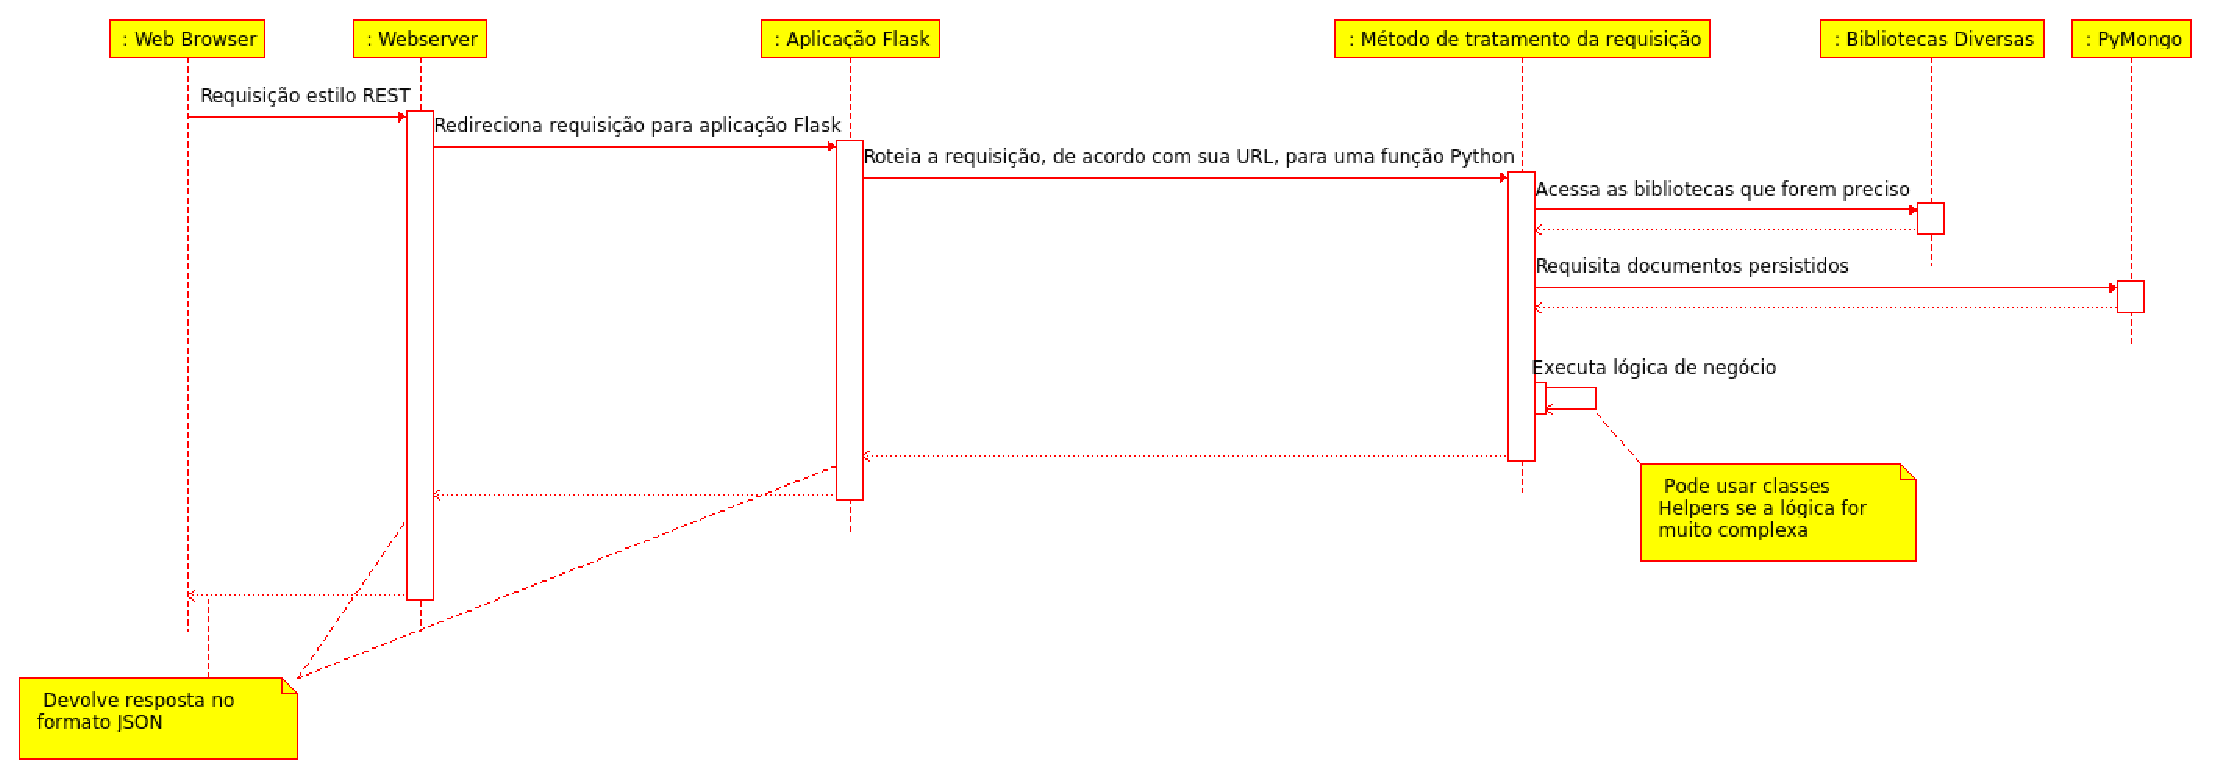
\includegraphics[width=15cm]{figuras/camada_api.eps}
	\caption{Camada \emph{REST WEB API}.}
	\label{camada_api}
\end{figure}

Tudo começa quando um \emph{browser web} faz uma requisição do tipo \emph{HTTP} a um servidor \emph{web}. 
O servidor \emph{web} identifica se a requisição é para a aplicação \emph{flask} do sistema em questão. 
Se for, esta requisição é repassada para a aplicação \emph{flask}. 
Agora as coisas começam a ficar mais interessantes. 
A aplicação \emph{flask} analisa a \emph{URL} da requisição, verifica o método da requisição e repassa os dados da requisição, num formato amigável ao \emph{python}, para uma função \emph{python}. 
Por padrão os parâmetros das requisições via método \emph{``GET"} são repassadas ao \emph{python} como \emph{string}. 
Para os demais métodos, padronizou-se receber o \emph{payload} da requisição \emph{HTTP}, como objetos JSON, que são facilmente convertidos para dicionários \emph{python}.

São nas funções \emph{python}, que tratam as requisições, que a lógica de negócio é executada. 
Aqui bibliotecas como a \emph{NumPy} podem ser chamadas, ou mesmo bibliotecas criadas pelos desenvolvedores da aplicação. 
É a partir deste ponto que dados podem ser acessados do banco de documentos pela biblioteca \emph{PyMongo}. 
Ao final da execução uma resposta é gerada no formato \emph{JSON} para que seja consumida pela camada \emph{web}.

A Figura \ref{webapi_componentes}, mostra um exemplo de componentes escritos em \emph{Python}, tratando uma requisição \emph{HTTP}, no caso uma chamada a \emph{URL http://<<myurl>>/patient}.
Depois que o servidor \emph{web} repassou a requisição para a aplicação que usa o \emph{framework Flask}, o \emph{framework} executa sua rotina de roteamento e descobre qual função \emph{Python}, contida no componente \emph{views},  deve ser executada, no caso a função \emph{get\_patients}.
Esta função acessa um objeto do tipo \emph{DataBase}, pertencente a biblioteca \emph{PyMongo}, e executa o método \emph{find} da coleção \emph{patients} pertencente ao \emph{DataBase}.
O resultado desta chamada são os dados contidos no banco de dados retornados no formato \emph{BSON}.
O componente \emph{json\_util}, da biblioteca \emph{PyMongo}, tem seu método \emph{dumps} chamado.
Este método converte os dados de \emph{BSON} para \emph{JSON}.
Finalmente, o \emph{framework Flask} responde a requisição.


\begin{figure}[ht]
	\centering
	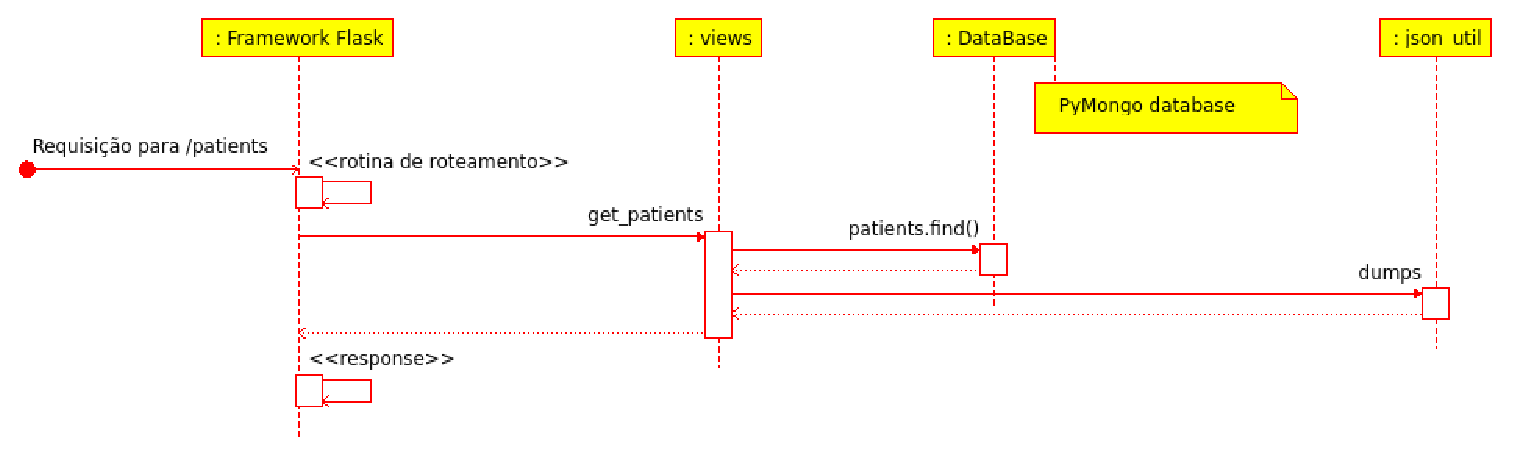
\includegraphics[width=17cm]{figuras/webapi_componentes.eps}
	\caption{Exemplo de requisição sendo tratada pela \emph{web api}.}
	\label{webapi_componentes}
\end{figure}

\subsection {CAMADA DE BASE DE DOCUMENTOS}

Para esta camada foi escolhido o banco de documentos \emph{MongoDB}, ver a seção \ref{mongodb_sec}. 
Há várias vantagens no uso desta tecnologia, mas a determinante foi a facilidade de uso e criação de estruturas de dados. 
No início do projeto, foi usado um banco de dados relacional e um \emph{framework} de mapeamento objeto-relacional. 
Devido a natureza altamente complexa dos dados, dados espaciais provindos de marcadores de superfície capturados por câmeras, eles são multidimensionais também. 
Sem dúvida isto ajudou a tornar possível criar esta primeira versão do software em tão pouco tempo.

A estrutura do banco da aplicação é mostrada na Figura \ref{mongo_oga}. 
O banco é composto por duas coleções: os dados dos pacientes na coleção \emph{patients} e os dados recuperados do \emph{QTM} \emph{positionals\_data}.

\begin{figure}[H]
	\centering
	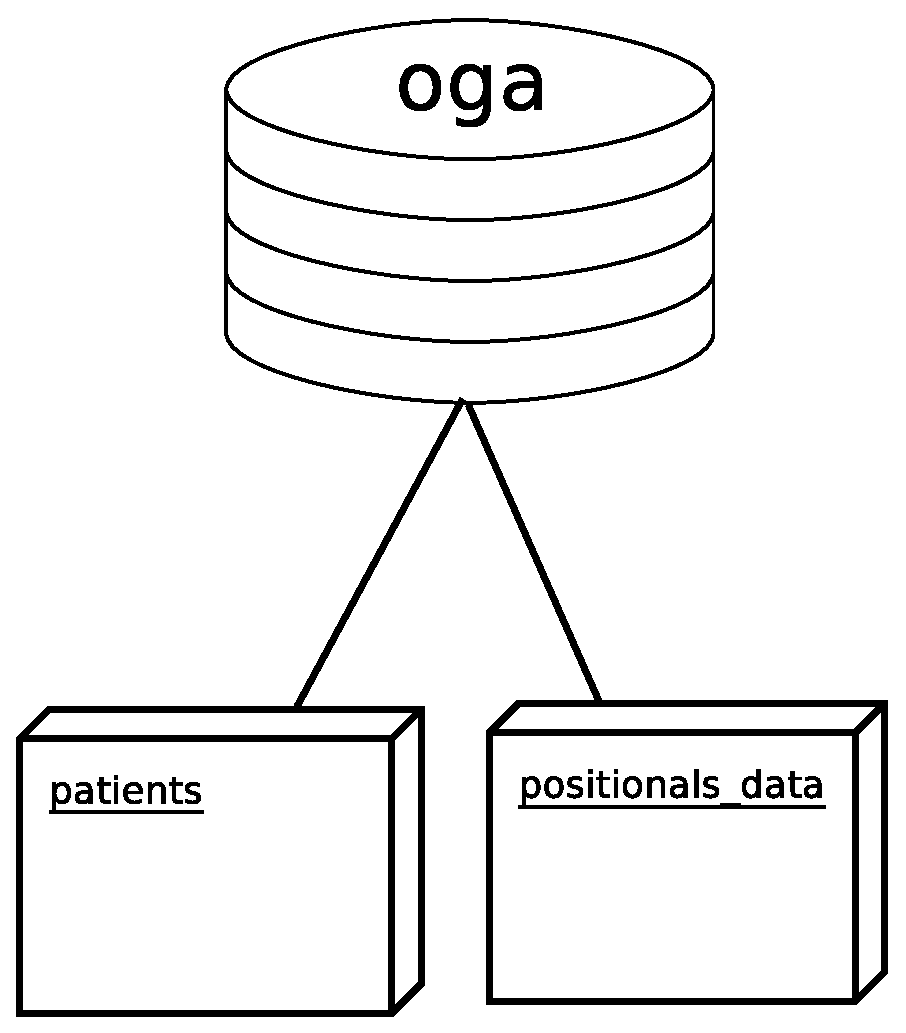
\includegraphics[width=5cm]{figuras/mongo_oga.eps}
	\caption{Banco de documentos da aplicação.}
	\label{mongo_oga}
\end{figure}

A Figura \ref{listagem2}  mostra um exemplo de documento da coleção \emph{patients}.
Já a Figura \ref{listagem3}  mostra um exemplo de documento da coleção \emph{positionals\_data}.

\begin{figure}[H]
	\centering
	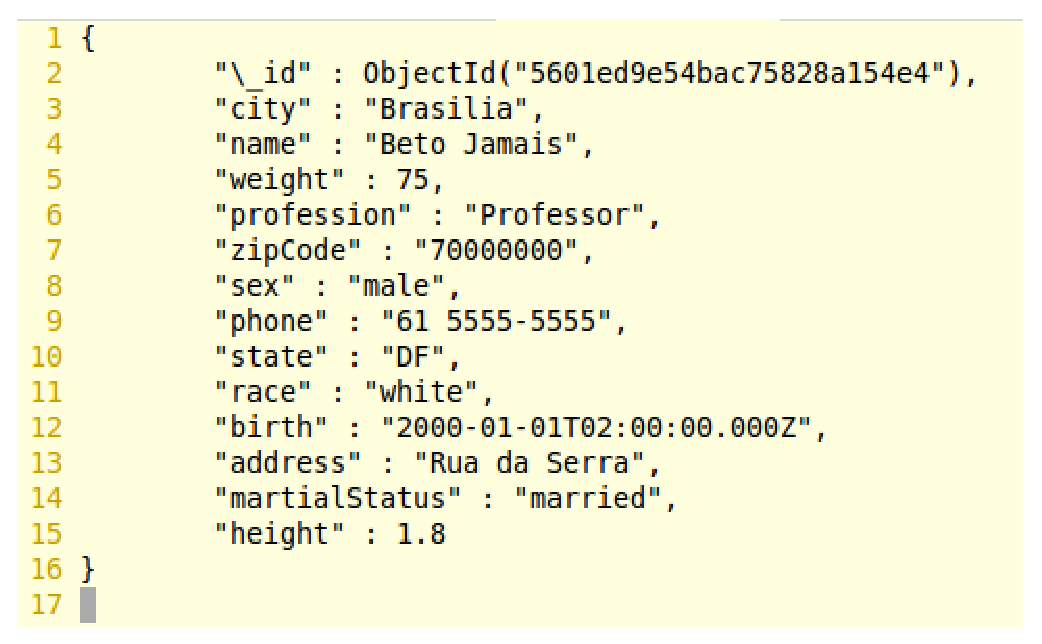
\includegraphics[width=10cm]{figuras/listagem2.eps}
	\caption{Documento da coleção \emph{patients}.}
	\label{listagem2}
\end{figure}

\begin{figure}[H]
	\centering
	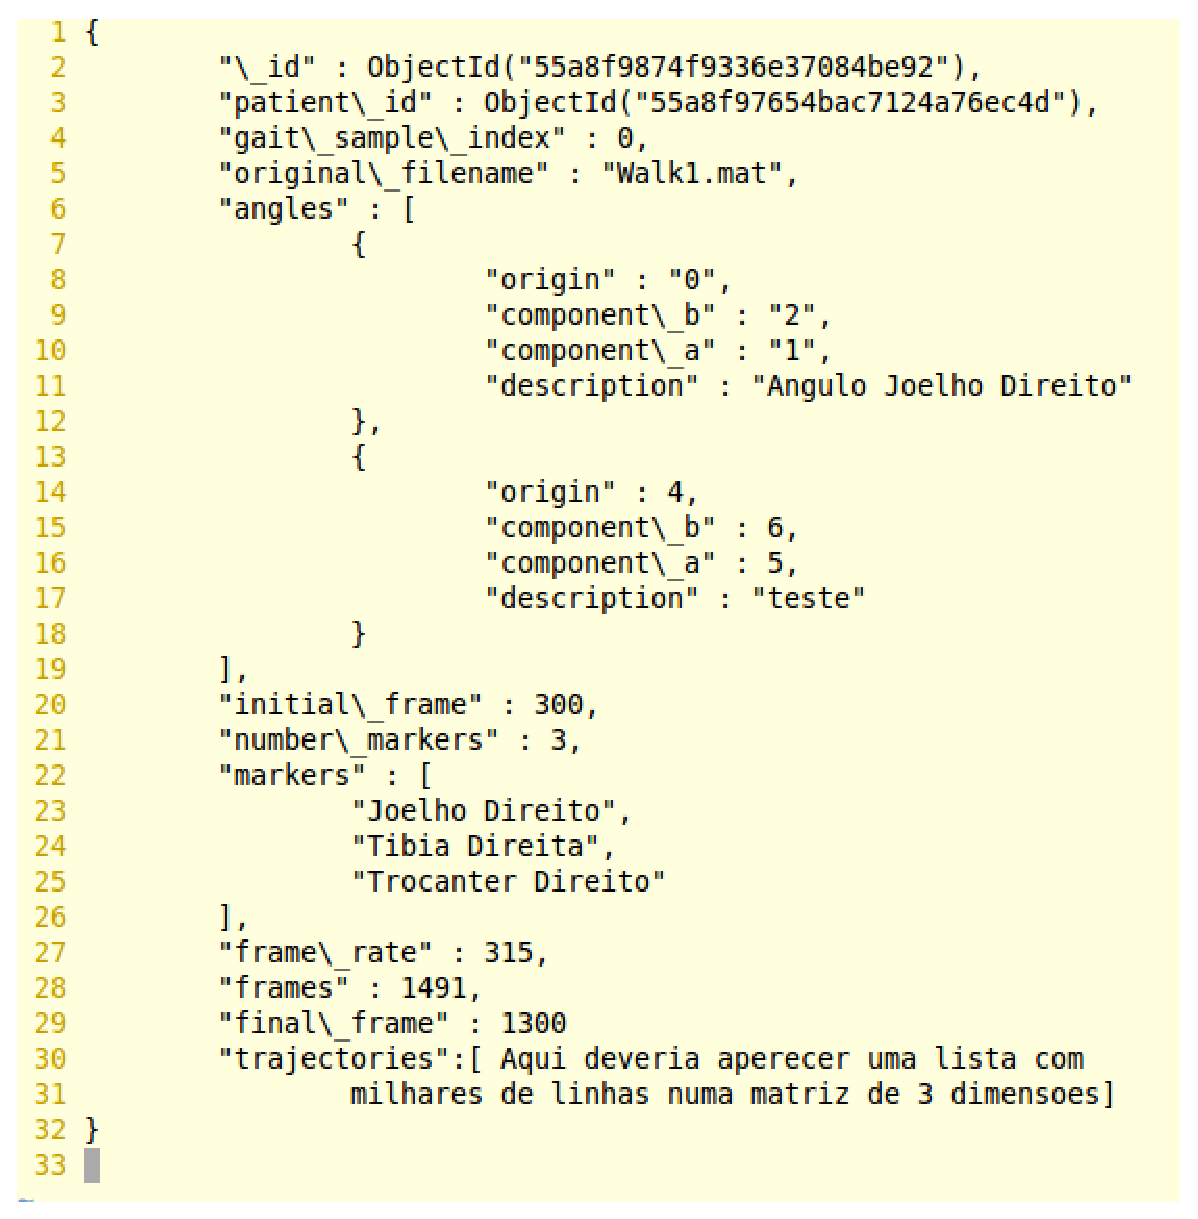
\includegraphics[width=10cm]{figuras/listagem3.eps}
	\caption{Documento da coleção \emph{positionals\_data}.}
	\label{listagem3}
\end{figure}


